% \subsection{Teknologianalyse}
% \label{sec:teknologianalyse}
% Vi ser en tydelig mulighed for at assistere forbrugere med at træffe et valg, når det kommer til køb af varer på nettet, bestemmelse af optimale lysforhold i hjemmet og visualisering af et tilkøbt element i forbrugernes dagligdag/hjem. Dette vil sandsynligvis kunne løses ved hjælp af bedre købsvejledning eller værktøjer til at assistere forbrugeren i en købssituation hvor en prøve ikke kan stilles til rådighed eller at returnere varen er umuligt eller for omfattende en process.

% % // redegørelse
% Blot at vælge en lampe fra et katalog er problematisk, hvis der ikke er billeder af lampen som
% \begin{enumerate}
%     \item Fremviser lampen som møbel, rent visuelt, det fysiske design og 
%     \item Viser hvordan lys kastes af lampen. En god løsning vil være at have en fysisk model placeret i en kontekst hvor man kan komme og se lampen og se lyset i sammenspil med anden indretning, således som f.eks. Ikea gør.
% \end{enumerate}

% Man vil også kunne skabe billige prototyper af lamper vha. 3D printer teknikker. Disse ville eventuelt være mulige at tage med hjem for at teste hvordan en lampe passer ind i det rum den egentligt er købt til, men fordi plastik vejer mindre end metal, glas og andre tunge materialer som lamper kan være produceret af, kunne man forestille sig ophængsmetoder der ikke nødvendiggør at bore huller i vægge, før man har set om lampen passer ind i rummet.

% En tredje metode kunne være at konstruere en 3D model af lampen og køre en simulation af, hvordan den kaster lys. Dette koncept vil også kunne udvides til, at en forbruger kan modellere deres eget hjem og placere lampen i den model af deres hjem som de opstiller. Eller det kan anvendes af sælgere som et værktøj til at vejlede forbrugeren til at påtage det rigtige køb.

% Indledning over

\subsection{Teknologier til visualisering}
Vi ser en tydelig mulighed for at assistere forbrugere med at træffe et valg, når det kommer til køb af varer på nettet. For at undersøge hvilke teknologier, der kan anvendes til visualisering, er der i dette afsnit en række teknologier og metoder, som alle er relevante i forhold til at visualisere en lampe. Teknologierne er udvalgt på baggrund af diskussion i gruppen, hvor mindre relevante teknologier, som f.eks. 3D-print blev fravalgt. Formålet med afsnittet er, at få en forståelse af hvilke teknologier der allerede eksisterer inden for visualisering, og finde ud af hvilke metoder, der er bedst i forhold til visualisering af lamper for brugere der handler via internettet.

\subsubsection{Digitale billeder taget med et fysisk kamera}
Som beskrevet under afsnit \ref{sec:ehandel}, benytter e-butikker, sig ofte af billeder til at vise kunden deres varer over internettet. Et eksempel på dette er vist på figur \ref{fig:e_handel_lampebilleder}.

\begin{figure}[H]
    \centering
    \fbox{\rule{\textwidth}{5cm}}
    \caption{Billeder af lamper på e-butikken somelampstore.what}
    \label{fig:e_handel_lampebilleder}
\end{figure} 

I det viste tilfælde er visualiseringen skabt ved at tage billeder af lamperne med et kamera fra en bestemt vinkel, i en kontekst, der typisk hænger sammen med lampetypen. 

Fordelen ved denne type af visualisering er, at den giver et virkelighedstro billede af, hvordan lampen ser ud i den kontekst, som billedet er taget i. Ulempen er, at der ofte kun er et begrænset antal billeder til rådighed, hvilket kan medføre, at forbrugeren ikke kan se lampen fra alle vinkler og på den måde ikke kan visualisere lampen for sig. Derudover kan det være svært, at se hvordan lyset udbreder sig fra lampen, da dette til dels afhænger af hvilken vinkel man ser lampen fra. 

Herudfra kan man kortfattet sige, at visualisering af lamper gennem billeder, taget med et fysisk kamera, giver et realistisk billede af lampen, men kun i den kontekst og vinkel billedet er taget i. 

% \subsubsection{3D print}
% En teknologi, som sælgeren vil kunne bruge, er 3D printere. 3D printere anvender plastik istedet for blæk, som bliver varmet op til knap 200 grader \cite{hvordan_3Dprinter}. Den flydende plastik bliver lagt i tynde lag og størkner hurtigt efter at have bundet sig med det underliggende lag. 

% Sælgeren kan give forbrugeren en fil, så forbrugeren selv vil være i stand til at lave et 3D print af en bestemt lampe. Dette forudsætter dog, at forbrugeren har en 3D printer og, at brugeren er dedikeret nok til at få printet lampen, da store objekter kan tage dage at printe og ofte skal deles op i mindre dele.\cite{hvordan_3Dprinter}. Derudover er 3D printere stadig en så ny teknologi, og de er stadig primært rettet mod hobbyfolk som vil bruge lang tid på, at få kallibreret printeren korrekt, da et print ellers nemt kan fejle. 3D printer er heller ikke en billig inverstering, da nogle modeller koster over titusinde kroner\cite{3D_printer}. 

% Idag vil det være en dårlig ide for sælgere at forvente, at deres kunder har en 3D printer derhjemme. Et andet problem er, at sælgeren også kommer i et dilemma, da sælgeren skal bestemme om man kan udgive tegninger inden forbrugeren har købt lampen eller om de skal betale en form for depositum.

\subsubsection{Computergrafik}
I computergrafik, er en 3D model, en beskrivelse af objekters form og materiale.\cite{computergrafik_introduktion} Computergrafiske metoder kan bruges til at immitere hvordan lys interaktere med modellen og på den måde tegne et billede af modellen. Der eksisterer en mængde forskellige computergrafiske metoder, flere af hvilke kan bruges sammen med andre for, at opnå et mere realistisk eller effektivt resultat. Der findes flere produkter som kan visualisere produkter til salg på websites som f.eks. Cylindo\cite{Cylindo}. Men vi har ikke kendskab til at andre specialisere sig, eller markedsføre sig på nuværende tidspunkt med deres kompetencer med fokus på visualisering af lampers belysning.

\paragraph{Rasterisering}
[FIND KILDER](Rasterisering er en metode til at visualisere miljøer med høj aktiv brugerinteraktion som f.eks. computerspil.\ref{rastarization} Metoden virker ved rent mattematisk at projektere modellen på et billedplan som repræsentere skærmen.\ref{rastarization}. Fordelen ved resterisering er at disse projektioner, kan foretages meget hurtigt af computerens grafikkort, som bygget specielt til formålet\ref{rastarization}. Dette kan dog mindske fleksibiliteten, og muligheden for mere avancerede visualisering, hvor der kræves refleksioner og refraktioner af lys, som ikke passer ind i den proces (graphics pipeline\ref{rasterization}, som de enkelte grafikkort danner billeder ud fra. 

[OMSKRIV SÅLEDES AT RADIOSITY GÅR IND UNDER RAYTRACING](\paragraph{Ray tracing \cite{raytracing_for_begyndere}}
Raytracing forsøger at simplificerer den fysiske model af lys ved at ignorere det lys som ikke rammer vores øjne. Raytracing er dog alligevel blandt de metoder som kendes for at kunne skabe de mest fotorealistiske renderinger. Dette gøres ved såkaldt \textit{backwards raytracing}, hvorved man følger en stråle fra øjet og ud mod 3D modellen, så tjekkes der for kollisioner mellem strålen og objekterne i modellen. Ved hver kollision kan man vælge at følge yderligere stråler som kan hjælpe med at udregne reflektioner eller komplekse skygger. Denne metoder står i modsætning til hvad man kalder \textit{forwards raytracing} som er den mere fysisk korrekte metode, hvor man følger stråler af lys fra hver lyskilde.

I forhold til rasterisering, tager raytracede billeder væsentligt længere tid at tegne, men komplekse lysfænomener som refleksioner og lys forvrængninger igennem semitransparante medier som vand(kaldet refraktion) er simple at beskrive for en raytracing algoritme, som kan tegne disse med realistisk precision. Nogle fænomener som bløde skygger kan også beskrives men jo flere typer fænomener og jo større realisme der kræves des længere tid tager det at tegne et billede, men raytracing tillader stor fleksabilitet.

\paragraph{Radiosity \cite{radiosity_by_wpi,radiosity_by_uob}}
Radiosity er hvad man kunne kalde en forwards raytracing metode. Her eksistere lyskilder ikke som specielle objekter i en 3D model, hvilket er tilfældet for de andre metoder, men her som objekter uden forskel fra de andre i modellen.

I radiosity modellen er alle flader betegnet med en absorbans faktor og en energi faktor. Absorbansen beskriver hvor meget af lys der rammer fladen der bliver absorberet. Absorberet lys hæver en flades energi og som i virkeligheden, afgives noget af den energi som lys, mens andet bliver omdannet til f.eks. varme. Lyskilder er således blot flader som starter med en mængde energi.

Radiosity er i stor grad blandt de mest tidskrævende metoder eftersom at den laver beregninger som ikke nødvendigvis bliver set i et billede. Dette muliggøre dog at visualisere en scene en gang og derefter at kunne se den fra mange vinkler eftersom at de ekstra udregninger allerede er gjort. Radiosity er derimod ikke designet til at håndtere fænomener som er afhængig af hvor man ser et objekt fra, så som reflektion og refraktion. Dvs. at radiosity ikke kan håndtere metalliske overflader eller semitransparante materialer. Til gændgeld er Radiosity rigtig god til at simulere matte overflader og skygger.)

\subsubsection*{Opsummering}
[OMFORMULER OG GØR MERE KLART](Billeder af den fysiske lampe er en god og nem løsning på visualiseringsproblemet, men computergrafik vil gøre det muligt for forbrugeren, at se lampen fra flere vinkler, hvor det måske er et større besvær for sælgeren at skaffe flere billeder af produktet istedet for blot at andvende en 3D model af lampen. Computergrafik giver også mulighed for nemt, at se lampen i forskellige kontekster ved at udskifte miljøet som lampen bliver renderet i. )

Ideen om at printe en model af en lampe fra en e-butik for at se hvordan den rigtigt ser ud er ikke en fornuftig løsning på nuværende tidspunkt, eftersom at 3D printere stadig er dyre og kan være svære at kalibrere korrekt. Computergrafik kan derimod nemt indlejres i en hjemmeside. Hvilken Computergrafisk teknik der er den korrekte er et case til case valg eftersom det helt afhænger af hvor meget fleksibilitet versus kvalitet der er nødvendigt. Rasterisering og radiosity kan begge implementeres på en måde hvorved der opnås et højt niveau af bruger interaktion som kan gøre værktøjet mere naturligt at anvende for forbrugeren. Eftersom at målet er at simulere lamper og ikke møbler som borde og stole, er langt mere komplekst at lave en god visualisation med rasterisering. Radiosity falder også til kort hvis der er behov for mere komplekse materialer som metalliske overflader eller f.eks. klar plast og glas. Billeder tegnet med raytracing kan tage lang tid at rendere, men der er mulighed for stor fleksibilitet og komplekse materialer er relativt simple at rendere. Med det grundlag vil rapporten fremadrettet arbejde med raytracing som metode til visualisering.

\subsection{Afgrænsning af løsningsfelt}
For at visualisere hvilken afgrænsning af løsningsfeltet, der nu er foretaget, har vi, ud fra ovenstående problemanalyse, fremstillet figur \ref{fig:p1_skitser}, der viser løsningsfeltet for det initierende problem. Figuren viser på den lodrette akse hvem der styrer visualiseringen af lamper, og den vandrette akse viser, hvor lamperne visualiseres. I feltet er fire løsningsmuligheder vist.

\begin{figure}[H]
  
  \centering
  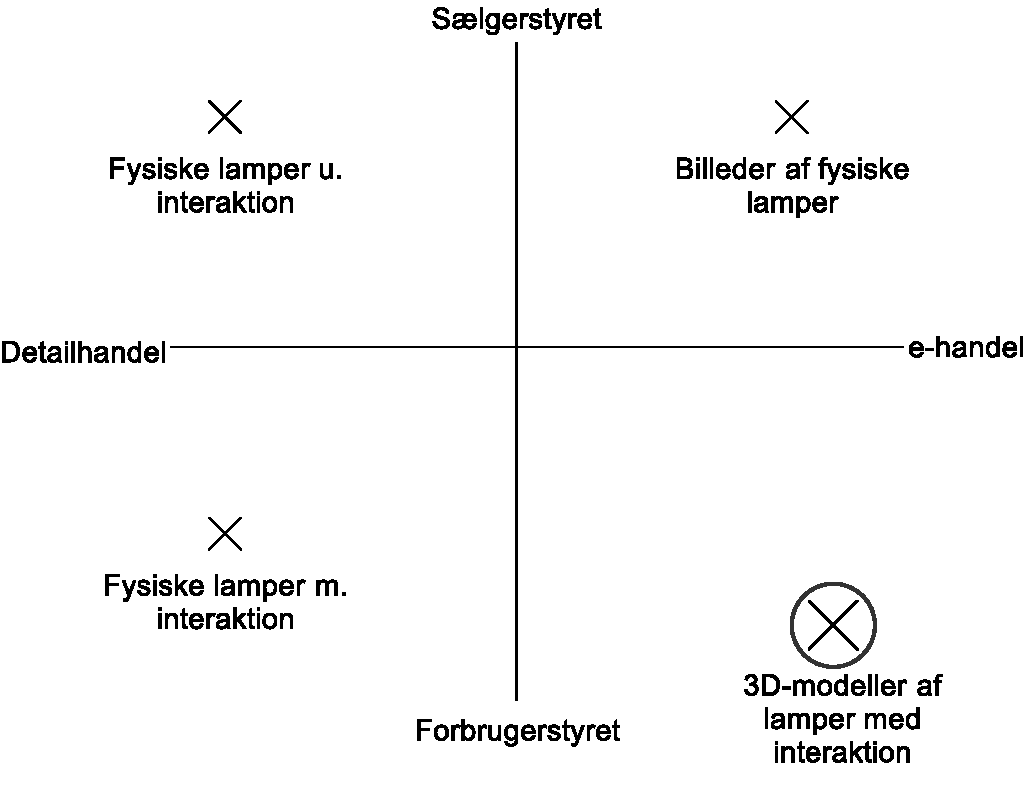
\includegraphics[width=10cm]{p1_skitser}
  \caption{Illustrerer lønningsfeltet til initierende problem, hvor det afgrænsede løsningsfelt er markeret med en cirkel.}
  \label{fig:p1_skitser}
\end{figure}

Herunder er de fire løsningsmuligheder, vist på figur \ref{fig:p1_skitser}, beskrevet:
\begin{enumerate}
  \item fysiske lamper uden interaktion, som er de lamper sælgeren udstiller i fysiske butikker, men som forbrugeren ikke har mulighed for interaktion med, det vil sige at dette ofte er lamper som er slukket.

  \item fysiske lamper med interaktion, som er de lamper sælgeren udstiller i fysiske butikker og som brugeren bla. kan slukke og tænde for, altså have interaktion med.

  \item billeder af fysiske lamper på e-butikker. Her har kunden mulighed for at se et billede af lampen, men kun fra de vinkler og i den kontekst som sælgeren har valgt.

  \item 3D-modeller af fysiske lamper m. interaktion på e-bukker. Her har kunden mulighed for at se et 3D billede af lampen samt rotere lampen, og herved se hvordan lampens belysning er fra de ønskede vinkler, og ikke kun i den kontekst som sælgeren vælger det. 
\end{enumerate}

Figuren viser nu at det er løsningsmulighed 4, som der afgrænset til i løbet af problemanalysen, og vi dermed har fravalgt løsningsmulighed 1-3 på baggrund af problemanalysen. Dette gør at der nu kan opstilles en endelig problemformulering, som ligger op til en løsningsmulighed 4.